\documentclass[conference]{IEEEtran}

%\renewcommand{\baselinestretch}{1.001}

% Pacote para escrever matrizes
\usepackage{amsmath}
\usepackage{graphicx}
\usepackage{array}
\newcolumntype{L}[1]{>{\raggedright\let\newline\\\arraybackslash\hspace{0pt}}m{#1}}
\newcolumntype{C}[1]{>{\centering\let\newline\\\arraybackslash\hspace{0pt}}m{#1}}
\newcolumntype{R}[1]{>{\raggedleft\let\newline\\\arraybackslash\hspace{0pt}}m{#1}}

%Package for the DOI paper insertion
% DOI
%\acmDOI{10.18293/SEKE2021-108}
\usepackage{textpos}
\usepackage{comment}

\usepackage{authblk}
\renewcommand*{\Authand}{\authorcr}
\renewcommand*{\Authands}{\newline} %%new line after each author
\renewcommand*{\Affilfont}{\normalsize}
\renewcommand*{\Authfont}{}    % make author names boldface    
\setlength{\affilsep}{0.1em}   % set the space between author and affiliation

\pagenumbering{gobble}
\usepackage{fancyhdr}
\renewcommand{\headrulewidth}{0pt}
\fancypagestyle{doi}{\lfoot{DOI reference number: 10.18293/SEKE2021-108}}

\begin{document}

\title{A Comparative Study of Psychometric Instruments in Software Engineering}

\author[1]{G. Guimarães}
\author[1]{M.Perkusich}
\author[1]{D. Albuquerque}
\author[2] {E.n Guimarães}
\author[1]{H. Almeida}
\author[1]{D. Santos}
\author[1]{A. Perkusich}
\affil[1]{Federal University of Campina Grande - Intelligent Software Engineering Group (ISE/Virtus) - Paraiba, Brazil}
\affil[2]{The Pennsylvania State University - Malvern, Pennsylvania - USA}



\maketitle
\thispagestyle{doi}
\begin{abstract}

Over the years, researchers have explored the influence of human factors in software engineering, showing that the team members' personalities might affect teamwork. However, it is challenging to measure software engineers' personalities due to the number of available psychometric instruments and the possibility of using different scales and classifications. Our study compares the personality traits measured by three psychometric instruments used in Software Engineering: Big Five Inventory (BFI), 16 Personality Factors (16PF), and Context Cards (CC). For this purpose, we executed an empirical study in which we collected data from 29 software developers for each of the evaluated instruments. As a result, we identified a moderate correlation between BFI and 16PF, confirming the current state-of-the-art. For the remaining combinations, there was a weak correlation. As implications for this research, there is a need to empirically evaluate BFI and CC (context-specific survey) in terms of construct validity since they have moderate to low correlation.

\end{abstract}

\begin{IEEEkeywords}
Human Aspects, Social Aspects, Personality, Software Engineering, Psychometric Instruments.
\end{IEEEkeywords}


\section{Introduction}

The success of software development projects is directly related to the team members’ technical (a.k.a. Hard skills) and non-technical skills (a.k.a Soft Skills) \cite{canedo2019factors}. Soft skills are becoming more important in the industrial environment because they affect team cohesion and team climate~\cite{gilal2017effective, ruiz2019understanding}, impacting its productivity and outcomes' quality~\cite{gomesevaluating, Iqbal2019BigfivePT}. 

A key aspect of studying soft skills is personality. Many studies investigated the effects of personality on teamwork performance in the last forty years~\cite{cruz2015forty, soomro2016effect}. These studies used several psychometric instruments to evaluate personality types and personality traits of software engineers~\cite{yilmaz2017examination, cruz2015forty, soomro2016effect}. The studies mostly used the Myers-Briggs Type Indicator (MBTI) or tests based on the Big Five (BF), such as Big Five Inventory (BFI) and Revised NEO Personality Inventory (NEO-PI-R). However, other psychometric instruments were also used, such as International Personality Item Pool (IPIP), the Sixteen Personality Factor Questionnaire (16PF), and Context-Specific Survey Instrument (Context Cards) \cite{cruz2015forty}. %\footnote[]{Corresponding author: gleyser.guimaraes@virtus.ufcg.edu.br}

Choosing a psychometric instrument is not straightforward because some require training and a license to be used. Moreover, McDonald and Edwards reported misuse of personality tests in software engineering (SE)~\cite{mcdonald2007should}. They argued that the inappropriate use of psychological tests and fundamental misunderstandings of personality theory caused a lack of progress in this field. Additionally, Graziotin et al. \cite{graziotin2020behavioral} demonstrated a deeper confusion on assessing related constructs using personality tests. For example, Capretz and Ahmed~\cite{capretz2010making} considered that the introvert trait is suitable for the programmer role, whereas Gorla and Lam~\cite{gorla2004should} concluded that it is the Extrovert trait. 

Having reliable data is the most critical factor for any SE measurement approach. Such observation is also valid for psychometric instruments. The inadequate application of psychometric instruments and their interpretation might lead to invalid results, economic loss, and harm to individuals. If the psychometric instruments or their usage are not valid, all the resulting conclusions are also invalid. Psychometric instruments measure latent variables (i.e., unobservable constructs) such as intelligence, personality, and happiness. Therefore, evaluating the psychometric instrument used is crucial to ensure that the variables are measured correctly.

Cruz et al.~\cite{cruz2015forty} discusses the existence of many disagreements in the SE research community regarding (i) the application of psychometric instruments and (ii) the interpretation of their results, comparing psychometric instruments' constructs to understand how to measure software engineers' personalities and their impact on productivity and quality. However, no other works are performing a similar comparison analysis in the past five years. 

Moreover, Gulati et al.~\cite{gulati2015comparative} examined studies based on human factors in software engineering. They compared studies relating to different personality instruments (i.e., MBTI, KTS, and BFI). Balijepally et al.~\cite{balijepally2006assessing} focused their research on comparing two emerging models, BFI and MBTI, for assessing personality traits in SE. To the best of our knowledge, these studies promote a discussion relating to software engineering and psychology but do not explore the correlation analysis among the personality instruments.

To address this gap, we investigated the similarity between three psychometric instruments: Big Five Inventory (BFI), 16 Personality Factors (16PF), and Context Cards (CC). We used these instruments because (i) studies in SE recurrently use them, (ii) they are of the public domain or readily available for researchers, (iii) they are clear to use in SE, and their data analysis have a vocabulary that is easy to understand, (iv) they do not have a large number of items, thus easing its execution and interpretation. We collected data from 29 subjects with about three to five years of experience in the area, and most of them were developers of web or mobile projects. We compared the instruments in terms of the number of questions, option type, response time, and the Kendall correlation.

This paper details the applied study and summarizes the results regarding the similarity of the evaluated psychometric instruments. The remainder of this paper is organized as follows.  Section~\ref{BACKGROUND} provides a background with an overview of psychometric instruments for SE. Section~\ref{Empirical Study} describes the study design. Section~\ref{Results and Discussion} presents the results and discusses the answers to the research questions.  Section \ref{THREATS TO VALIDITY} analyzes the study's threats to validity. Finally, Section~\ref{CONCLUSIONS AND FUTURE WORKS} presents our conclusions and directions to future work.












\section{Background and Related Work}
\label{BACKGROUND}

This section presents an overview of psychometric instruments and describes the studies that compared psychometric instruments in the context of Software Engineering.

\textbf{Psychometric Instruments Overview}. Personality involves different theoretical perspectives, definitions, and levels of abstraction. We used the personality definition established by Ryckman~\cite{ryckman2012theories}, in which it is defined as ``a dynamic and organized set of characteristics possessed by a person that uniquely influences his or her cognitions, motivations, and behaviors in various situations''. We used this definition due to its popularity in Software Engineering research. 

Psychometric instruments have been used to evaluate personality \textit{traits} and \textit{types} of individuals, usually by using questionnaires. Personality traits are stable characteristics of individuals such as being optimistic, sociable, and imaginative, whereas Personality types are constructs that indicate independent groups such as mediator, entrepreneur, and adventurer. For instance, using the 16PF psychometric instrument, a person that scores high on the traits ``introversion'', ``sensing'', ``thinking'', and ``judging'' would be classified as being of the personality type ``logistician''.

\textbf{Psychometric Instruments in SE}. Software development organizations use psychometric instruments to measure their members' personality~\cite{lounsbury2007investigation, wyrich2019theory}. The most used psychometric instruments in SE are based on the Big Five (BF) theory - e.g., Big Five Inventory (BFI) \cite{cruz2015forty}. Other psychometric instruments have been widely used in SE research, such as the 16 Personality Factor Questionnaire (16PF) and Context-specific survey instrument (CC). Next, we describe each of the aforementioned psychometric instruments.

\textit{Big Five Inventory (BFI)} describes the personality by employing broad factors (dimensions) of personality traits~\cite{costa2010neo}. Its five dimensions are Extraversion, Agreeableness, Conscientiousness, Neuroticism (a.k.a. Emotional Stability), and Openness to Experience (sometimes called Intellect or Imagination). The BFI-44 is a self-report inventory created to measure the Big Five dimensions. The psychometric instrument contains 44 items and consists of short and descriptive phrases that respondents rated on a 5-point scale ranging from strong disagreement to strong agreement. This method is not in the public domain. However, it is readily available for researchers to use for non-commercial research purposes. 

\textit{The 16 Personality Factor Questionnaire (16PF)} is a psychometric instrument to identify characteristics, personality traits, and behavior. 16PF was published in 1949 and has been used to evaluate personality in many contexts, including career assessment and SE \cite{gomesevaluating}. The 16PF online test comprises five personality dimensions, making up 16 personality types. 16PF has five aspects: Mind, Energy, Nature, Tactic, and Identity. 16PF generates 16 types of personalities by acronyms generated from the dichotomies emitted by the psychometric instrument's aspects. The combination of four personality aspects results in a personality type. For instance, the combination of Extroversion (E), Observant (S), Thinking (T), Judging (J), and Assertive (-A) result in the personality ESTJ-A.  The Identity scale (i.e., assertive or turbulent) is in all personality types because it affects other scales. As a result, when we considered this scale, the method describes 32 different personality types. 

\textit{Context-specific survey instrument (CC)} was proposed by Yilmaz et al.~\cite{yilmaz2017examination} aims to reveal and illustrate the personality characteristics of the individuals in software development teams. The instrument combines situations from companies with basic patterns (items) of the Big Five Inventories (BFI-44) questionnaire to create a card game-based personality identification method~\cite{yilmaz2017examination}. The context cards describe the human personality traits in terms of five fundamental factors: Extraversion, Openness, Agreeableness, Neuroticism, and Conscientiousness.  This model identified six themes (traits) for each factor, totaling 30 themes. For example, the factor Extroversion has the traits talkative, assertive, energetic, active, approachable, and outgoing.
 
 \textbf{Psychometric Instruments Evaluation in SE}. Next, we discuss studies that assessed psychometric instruments in SE. Jia et al.~\cite{jia2015comparative} reviewed and compared three psychometric instruments (i.e., BFI, MBTI, and KTS). They observed the number of questions, option type, and time spent answering the test. The researchers collected empirical evidence for comparison from articles published between 2010 and 2014. They concluded that BFI is the more suitable alternative to evaluate soft-skills in software development activities. 

Another study by Gulati et al.~\cite{gulati2015comparative} compared studies published between 2003 and 2014 that analyzed human factors in software engineering. They concluded that the most popular psychometric instruments in SE are MBTI and BFI. Finally, Balijepally et al.~\cite{balijepally2006assessing} dedicated their research mainly to compare BFI and MBTI. They suggested that BFI is more valuable than MBTI because BFI provides better measures for all MBTI factors, and it also evaluates Neuroticism, an important personality trait. 

Even though these studies promote a great discussion relating to software development activities (i.e., SE area) and soft-skills (i.e., Psychology area), they perform the models' comparison based solely on data available in the literature. Consequently, we conclude that these studies highlight the importance of human psychology in SE and realized conceptual comparisons but lack evidence about how the psychometric instruments compare in the context of SE. To address this gap, we compared personality instruments by collecting data from software developers and analyzing the correlation between the instruments' answers.
\section{Research Methodology}
\label{Empirical Study}

This section presents the research methodology for the empirical study, including research questions, subjects' profiles, experimental materials, and data analysis procedures.

\textbf{Objective and Research Questions}. Our study aimed to analyze and evaluate the correlation between three state-of-art psychometric instruments (i.e., BFI, 16PF, and CC) in the context of software development activities. Given this, we formulated some Research Questions (RQs):

\begin{itemize}
    \item {\bfseries RQ1:} To what extent do BFI dimensions correlate with 16PF  considering software developers' personality?
    \item {\bfseries RQ2:} To what extent do 16PF aspects correlate with CC factors considering software developers' personality?
    \item {\bfseries RQ3:} To what extent do BFI dimensions correlate with CC factors considering software developers' personality?
 \end{itemize}
 
\textbf{Subjects}. We applied the psychometric instruments with 29 software developers (24 men and five women) from one Brazilian software organization. This organization had approximately 250 employees and produced more than 40 projects in collaboration with multinational partners. The employees were organized into small agile teams (around five to ten members).

The participant's ages ranged from 21 to 29 years, with a mean of 24 years. They had an average of three years of experience with software development. They developed Web and mobile applications using different technologies (e.g., Javascript, Java, HTML). Overall, the subjects' profile meets our study assumptions since all of them work in software development.

\textbf{Experimental Materials}. We created a questionnaire \footnote{Available in https://bit.ly/38E6yhP} with five sections to apply the psychometric instruments and submitted it to the ethics committee from the Federal University of Campina Grande (UFCG) for analysis and approval before conducting the study. The ethics committee gave us the certification (02505718.0.0000.5182), meaning we could collect data using the questionnaire. In the following, we present information about the questionnaire.

The \textit{first section} of the questionnaire presented the study objectives and the consent form, as approved by the ethics committee. This section contained information to motivate the participants to participate in the study. The \textit{second section} contained questions to collect demographic data, including name, gender, experiences, and age. The \textit{third section} contained BFI-44 questions translated and adapted to Portuguese by Andrade~\cite{andrade2008evidencias}. We also consulted the BFI-44 in Portuguese available on the Berkeley Personality Lab site\footnote[2]{https://www.ocf.berkeley.edu/$\sim$johnlab/bfi.htm}. All questions were answered through a five-point Likert-type scale: 1 (Strongly disagree) - 5 (Strongly agree), expressing their agreement degree regarding the question's descriptions. The \textit{fourth section} contained 16PF questions. The 16PF has about 60 questions (statements), each of them to be answered through a seven-point Likert-type scale (from ``agree'' to ``disagree''). 

Finally, the \textit{fifth section} included the CC questions. We translated and adapted the Context Cards to Portuguese. This psychometric instrument includes 60 cards (e.g., situations, questions), in which each card presents a situation and two optional answers described by A and B. The optional answers describe SE situations. One example of the original text on the one card is presented next. Situation (``During a team base discussion...''), Option A (``Evidence suggests that what we learn is mostly from our conflicts.''), and Option B (``I believe compromise between people for a common ground more successful.''). Each person spends about 40 minutes - on average - to complete the questionnaire.

\textbf{Procedure}. We applied the questionnaire during the period that the software organization made available for the research. Before the questionnaire application, the study's authors ran a training session with the participants. The training session lasted 30 minutes, and the participants spent between 30 to 40 minutes answering the entire questionnaire. The training session aimed to present the questionnaires' concepts and level the participants' understanding regarding the psychometric instruments and study's goals. In other words, we motivated the participants to answer based on reality (not intentions) and understood the questions. Further, we emphasized that there were no ``correct'' answers and that they would not be identified. Such support minimized internal validity threats. 

\textbf{Analysis Procedure}. We defined the following criteria for comparing the psychometric instruments: the number of questions, option type, response time, and the correlation between the results (i.e., the correlation between the facets, dimensions, and aspects of psychometric instruments). The correlation analysis sought to verify the correlation between the personality traits presented by instruments for each participant. The BFI-44, 16PF, and Context Cards instruments contain different sets of Likert-type items combined into single composite scores (as explained in Section~\ref{BACKGROUND}). Thus, they calculate a score for each facet or dimension of the psychometric instrument. Each of these composite scores provides a quantitative measure of a personality trait. 

Considering that the variables measured in this study are ordinal, we used the Kendall correlation coefficient. Kendall correlation coefficient is a nonparametric measure of the strength and direction of the association between two variables measured on at least an ordinal scale~\cite{puth2015effective}. We also used the correlation coefficients interpretation for psychology described by Dancey and Reidy \cite{dancey2007statistics}.














\section{Results and Discussion}
\label{Results and Discussion}

This section presents the main results for the comparison between the three psychometric instruments. 

\textbf{Personality Test Results}. We obtained personality traits’ scores for each participant by applying the three psychometric instruments (i.e., BFI, 16PF, and CC). It is worth mentioning that each instrument provided a set of personality trait scores for each participant. We calculated these scores using the guidelines for each instrument. Next, we present the results when applying each psychometric instrument.

\textit{BFI results:} We found the following quantities of participants with the dimension value assessed above 50\%: Extraversion (20 participants), Agreeableness (29 participants), Conscientiousness (28 participants), Neuroticism (12 participants), and Openness to Experience (24 participants). 

\textit{16PF results:} We found more Extroverts (52\%) types than Introverts (48\%), more Sensing (55\%) than Intuitive (45\%), fairly more Feeling (65\%) than Thinking (35\%), and more Judging (65\%) compared to Perceiving (35\%) type. The personality types most present were ENFJ, ESFJ, and ISFJ. However, we did not have participants with the personality types ISTP, ESTP, INFJ, and ENTP. Considering the Identity scale, the personality type most present was ENFJ-A.

\textit{CC results:} We obtained the following quantities of participants with the factor value assessed above 50\%: Extraversion (17 participants), Agreeableness (27 participants), Conscientiousness (15 participants), Neuroticism (4 participants), and Openness to Experience (8 participants). 

We analyzed the number of questions, option type, and time to respond to the psychometric instruments compared. Considering the number of questions and option type, 16PF contains 60 7-point questions, BFI-44 contains 44 5-point questions, and CC contains 44 A or B questions. The participant's average response time was 12 minutes to 16PF, 10 minutes to BFI-44, and 15 minutes to CC. 

Nevertheless, in addition to these comparison criteria, we were interested in the correlation between the test results (i.e., the correlation between the facets, dimensions, and aspects of psychometric instruments). We discussed the analysis of this criterion by answering the research questions.

\textbf{RQ1 - To what extent do BFI dimensions correlate with 16PF aspects considering software developers’ personality?}. Aims to address this RQ, we applied Kendall’s correlation between 16PF dichotomies and BFI dimensions. The correlation results can be seen in Table~\ref{tabela3}.

\begin{table}[!h]
\centering
\caption{Correlation between 16PF Dichotomies
 and BFI Dimensions.}
\label{tabela3}
\scalebox{0.80}{
\begin{tabular}{c|ccccc|}
\cline{2-6}
\multicolumn{1}{l|}{}                    & \multicolumn{5}{c|}{\textbf{BFI}}                                                        \\ \cline{1-1}
\multicolumn{1}{|c|}{\textbf{16PF}}      & \textbf{Extrav.} & \textbf{Agree.} & \textbf{Openn.} & \textbf{Consc.} & \textbf{Neuro.} \\ \cline{2-6} 
\multicolumn{1}{|c|}{\textbf{Extrovert}} & \text{0.57}    & 0.23            & 0.29            & 0.40            & -0.17           \\ \cline{2-6} 
\multicolumn{1}{|c|}{\textbf{Feeling}}   & 0.04             & \text{0.53}   & -0.08           & 0.13            & -0.19           \\ \cline{2-6} 
\multicolumn{1}{|c|}{\textbf{Intuitive}} & 0.01             & -0.03           & \text{0.50}   & -0.27           & -0.05           \\ \cline{2-6} 
\multicolumn{1}{|c|}{\textbf{Judging}}   & 0.12             & 0.11            & -0.12           & \text{0.71}   & -0.08           \\ 
\cline{2-6} 
\multicolumn{1}{|c|}{\textbf{Assertive}} & 0.33    & 0.24            & 0.15            & \text{0.40}            & \text{-0.57}           \\
\hline
\end{tabular}}
\end{table}

Figure~\ref{fig2} shows the distribution of participants considering the 16PF's Extroversion dichotomy (16PF-E), 16PF's Introversion dichotomy (16PF-I), and the  BFI's Extraversion dimension (BFI-E). In the figure, each point represents the participant score (i.e., the score of dimension or facet) obtained from the psychometric instrument.

\begin{figure}[!ht]
\centerline{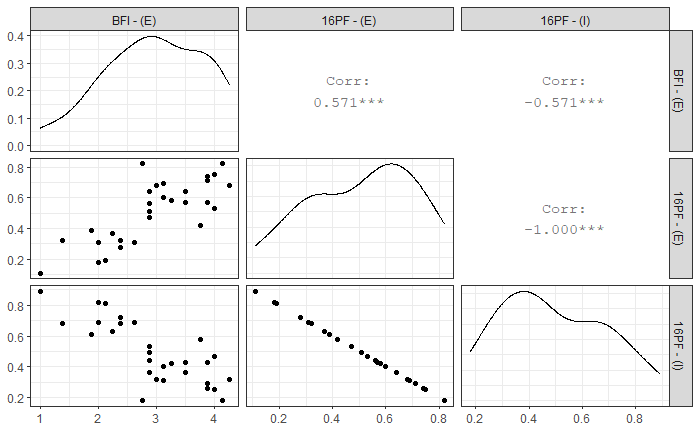
\includegraphics[scale=0.40]{Imagens/n1.PNG}}
\caption{The correlation coefficient between 16PF's Extroversion dichotomy (16PF-E), 16PF's Introversion dichotomy (16PF-I), and BFI's Extraversion dimension (BFI-E).}
\label{fig2}
\end{figure}

We found a moderate correlation between BFI's Extraversion dimension (BFI-E) and the 16PF's Mind aspect (16PF-E and 16PF-I). This correlation was positive to 16PF's Extroversion dichotomy (16PF-E) and negative to 16PF's Introversion dichotomy (16PF-I). The coefficient of 0.571 (p $<$  0.01) indicates a moderate positive correlation between 16PF-E and BFI-E. As expected, the correlation for 16PF-I was inversely correlated -0.571 (p $<$  0.01) with BFI-E. The results found reinforced the analysis performed by Jia et al.~\cite{jia2015comparative, balijepally2006assessing}, which stated that BFI's Extraversion dimension (BFI-E) is correlated to the 16PF's Extroversion dichotomy (16PF-E). 

%\begin{table}[http]
%\centering
%\caption{Personality Assessment Methods}
%\label{tabela1}
%\scalebox{0.70}{
%\begin{tabular}{|c|c|c|c|}
%\hline
 %                     & \textbf{\begin{tabular}[c]{@{}c@{}}Number\\ of questions\end{tabular}} %& \textbf{Option type}                                    & %\textbf{\begin{tabular}[c]{@{}c@{}}Average \\response time\end{tabular}} \\ \hline
%\textbf{16PF}          & 60                                                                    & %\begin{tabular}[c]{@{}c@{}}7-point\\ scale\end{tabular} & 12 minutes                                                            \\ \hline
%\textbf{BFI-44}  & 44                                                                     & %\begin{tabular}[c]{@{}c@{}}5-point\\ scale\end{tabular} & 10 minutes                                                             \\ \hline
%\textbf{Context Cards} & 60                                                                     %& A or B                                                  & 15 minutes                           %                                 \\ \hline
%\end{tabular}}
%\end{table}

Considering the distribution of participants for 16PF's Feeling dichotomy (16PF-F) and 16PF's Thinking dichotomy (16PF-T) and the BFI's Agreeableness dimension (BFI-A), We found a moderate correlation with a coefficient of 0.534 (p $<$ 0.01) between 16PF-F and BFI-A. As expected, the correlation between 16PF-T and BFI-A was inversely correlated. Also, we found a moderate correlation between BFI's Conscientiousness dimension (BFI-C) and the 16PF's Identity aspect. This correlation was positive to 16PF's Assertive dichotomy (16PF-A) and negative to 16PF's Turbulent dichotomy (16PF-T).

Similarly, we obtained a moderate correlation between BFI's ``Openness to Experience'' dimension (BFI-O) and the 16PF's Energy aspect (16PF-N and 16PF-S). This correlation was positive to 16PF's Intuitive dichotomy (16PF-N) and negative to 16PF's Observant dichotomy (16PF-S). The correlation coefficient of 0.502 (p $<$ 0.01) indicated a moderate correlation between the BFI-O and the 16PF's Intuitive dichotomy (16PF-N). As expected, the correlation coefficient was negative between the BFI's ``Openness to Experience'' dimension (BFI-O) and the 16PF's Observant dichotomy (16PF-S).  

Considering the 16PF's Judging dichotomy (16PF-J), 16PF's Prospecting dichotomy  (16PF-P), and the BFI's Conscientiousness dimension (BFI-C). The correlation coefficient of 0.712 (p $<$ 0.01) indicated a strong positive correlation between 16PF-J and BFI-C. As expected, the correlation between 16PF-P and BFI-A was inversely correlated -0.712 (p $<$ 0.01). We obtained a strong correlation between BFI-C and the 16PF's Tactic aspect (16PF-J and 16PF-P). This correlation was positive with 16PF-J and negative to 16PF-P.  

As in previous studies ~\cite{cattell2008sixteen,cattell1995personality, schneewind199816, gerbing199116pf} our study identified a strong correlation between 16PF-J and BFI-C.  However, we found a moderate correlation between 16PF-E and BFI-E, 16PF-F and BFI-A, and 16PF-N and BFI-O, unlike Cattell and Mead ~\cite{cattell2008sixteen}, which found a strong correlation. Additionally, we observed a weak correlation between 16PF-F and BFI-N. 

Further, we analyzed the correlation of 16PF's Identify aspect (16PF-A and 16PF-T) with BFI's dimensions. We obtained a coefficient of -0.578 (p $<$ 0.01) for the correlation between the 16PF's Assertive dichotomy (16PF-A) and BFI's Neuroticism dimension (BFI-N). Further, the correlation between (16PF-A) and BFI's Conscientiousness dimension (BFI-C) was 0.40 (p $<$ 0.01). Considering the 16PF's Turbulent dichotomy (16PF-T), we obtained a correlation coefficient of 0.580 (p $<$ 0.01) with BFI-N, and -0.416 (p $<$ 0.01) with BFI-C. Table~\ref{tabela3} illustrates the results of Kendall’s correlation between 16PF dichotomies and BFI dimensions. 
 
We concluded that BFI-C correlated strongly with 16PF-E. We found a moderate correlation between 16PF-E and BFI-E, 16PF-F and BFI-A, and 16PF-N and BFI-O. We found a weak correlation between 16PF-F and BFI-N. Further, 16PF-A correlated moderately with BFI-C (moderately positive) and BFI-N (moderately negative). Thus, we concluded that BFI and 16PF had a moderate correlation. 


\textbf{RQ2 - To what extent do 16PF aspects correlate with CC factors considering software developers’ personality?}.
Aims to address this RQ, we applied Kendall’s correlation between 16PF dichotomies and CC factors. The correlation results can be seen in Table~\ref{tabela45}. The correlation coefficient of 0.35 (p $<$  0.01) indicates a weak positive correlation between 16PF's Extroversion dichotomy (16PF-E) and the CC's Extroversion factor (CC-E). Additionally, we obtained a weak correlation between 16PF's Mind aspect (16PF-E and 16PF-I) and CC's Extroversion factor (CC-E).
Similar to what happens with 16PF and BFI.

\begin{table}[!ht]
\centering
\caption{Correlation between 16PF Dichotomies and context cards factors.}
\label{tabela45}
\scalebox{0.80}{
\begin{tabular}{c|ccccc|}
\cline{2-6}
\multicolumn{1}{l|}{}                    & \multicolumn{5}{c|}{\textbf{Context Cards}}                                              \\ \cline{1-1}
\multicolumn{1}{|c|}{\textbf{16PF}}      & \textbf{Extrav.} & \textbf{Agree.} & \textbf{Openn.} & \textbf{Consc.} & \textbf{Neuro.} \\ \cline{2-6} 
\multicolumn{1}{|c|}{\textbf{Extrovert}} & \text{0.35}    & 0.09            & -0.036          & -0.21           & 0.10            \\ \cline{2-6} 
\multicolumn{1}{|c|}{\textbf{Feeling}}   & 0.11             & 0.07            & 0.09            & -0.25           & \text{-0.34}  \\ \cline{2-6} 
\multicolumn{1}{|c|}{\textbf{Intuitive}} & 0.007            & -0.14           & 0.25            & -0.09           & 0.02            \\ \cline{2-6} 
\multicolumn{1}{|c|}{\textbf{Judging}}   & 0.19             & 0.14            & \text{-0.36}  & -0.008          & 0.05            \\ 
\cline{2-6} 
\multicolumn{1}{|c|}{\textbf{Assertive}} &0.29    & 0.27            & 0.02            & \text{-0.33}            & -0.08          \\
\hline
\end{tabular}}
\end{table}

Regarding 16PF's Judging dichotomy (16PF-J) and CC's ``Openness to Experience'' factor (CC-O), we found a negative correlation -0.36 (p $<$  0.01) between 16PF-J and CC-O.  Further, we found a weak correlation between CC's ``Openness to Experience'' factor (CC-O) and the 16PF's Tactic aspect (16PF-J and 16PF-P. Considering the 16PF's Feeling dichotomy (16PF-F) and CC's Neuroticism factor (CC-N), we observed a negative correlation coefficient of -0.34 (p $<$ 0.01), which indicated the weak correlation between these characteristics. Finally, we found a weak correlation between CC's Neuroticism factor (CC-N) and 16PF's Nature aspect (16PF-T and 16PF-F). Given the discussed results, we concluded that the correlation between 16PF and CC was weak.

\textbf{RQ3 - To what extent do BFI dimensions correlate with CC factors considering software developers’ personality?}. Aiming to address this RQ, we applied Kendall’s correlation between BFI dimensions and CC factors. The correlation results can be seen in Table~\ref{tabela5}. Considering the five characteristics analyzed for each psychometric instrument, we had a weak correlation (correlation coefficient of 0.38 (p $<$ 0.01)) between CC's Extroversion factor (CC-E) and BFI's Extraversion dimension (BFI-E). We found a correlation coefficient of 0.30 (p $<$ 0.01) between BFI's Conscientiousness dimension (BFI-C) and CC's Extroversion factor (CC-E). Further, we obtained a weak correlation between CC's Extroversion factor (CC-E) and the BFI's Extraversion dimension (BFI-E). 
CC's Conscientiousness factor (CC-C) had a correlation coefficient of -0.34 (p $<$ 0.01) with BFI's Agreeableness dimension (BFI-A) and 0.32 (p $<$ 0.01) with BFI's Neuroticism dimension (BFI-N). Thus, we concluded that there was a weak correlation between CC's Conscientiousness factor (CC-C) and the BFI's Agreeableness dimension (BFI-A) and BFI's Neuroticism dimension (BFI-N).  


\begin{table}[!ht]
\centering
\caption{Correlation between BFI Dimensions and context cards factors.}
\label{tabela5}
\scalebox{0.80}{
\begin{tabular}{c|ccccc|}
\cline{2-6}
\multicolumn{1}{l|}{}                  & \multicolumn{5}{c|}{\textbf{Context Cards}}                                              \\ \cline{1-1}
\multicolumn{1}{|c|}{\textbf{BFI}}     & \textbf{Extrav.} & \textbf{Agree.} & \textbf{Openn.} & \textbf{Consc.} & \textbf{Neuro.} \\ \cline{2-6} 
\multicolumn{1}{|c|}{\textbf{Extrav.}} & \text{0.38}    & 0.04            & -0.02           & -0.21           & 0.002           \\ \cline{2-6} 
\multicolumn{1}{|c|}{\textbf{Agree.}}  & 0.28             & 0.27            & -0.09           & \text{-0.34}  & -0.30           \\ \cline{2-6} 
\multicolumn{1}{|c|}{\textbf{Openn.}}  & 0.15             & -0.08           & 0.12            & -0.21           & 0.19            \\ \cline{2-6} 
\multicolumn{1}{|c|}{\textbf{Consc.}}  & \text{0.30}    & -0.08           & -0.21           & -0.09           & 0.04            \\ \cline{2-6} 
\multicolumn{1}{|c|}{\textbf{Neuro.}}  & -0.12            & -0.24           & -0.02           & \text{0.32}   & 0.16            \\ \hline
\end{tabular}}
\end{table}


Despite measuring similar characteristics, we concluded that the relationship between BFI and CC is weak. These results are not similar to those found by Yilmaz at el.~\cite{yilmaz2017examination}, in which the authors proposed and validated CC. In this study, they proposed results that assumed a strong correlation between the use of CC and BFI. Such correlations were the CC's Extroversion factor (CC-E) with the BFI's Extraversion dimension (BFI-E) (correlation coefficient of 0.93). They also found a strong correlation between CC's Conscientiousness factor (CC-E) and BFI's Conscientiousness dimension (correlation coefficient of 0.79).

We believe that a possible explanation for such distinction between the study findings and Yilmaz et al.'s~\cite{yilmaz2017examination} maybe the loss of semantics aspects from the original CC (once the originals were written in English language and the ones applied here were translated into Brazilian Portuguese). Besides that, the cultural factor may have influenced the interviewees' understanding of some questionnaire items' situations. We concluded that CC inventory is currently lacking independent replications to validate its reliability. In sum, this highlights the importance of developing such research in the SE field to enhance the surveys and studies that approach psychometric aspects and team formation. 












































\section{Threats to Validity}
\label{THREATS TO VALIDITY}

This section discusses the study's threats to validity following the classification proposed by Wohlin et al. ~\cite{wohlin2012experimentation} and the strategies applied to mitigate them.

\textit{Internal validity:} We applied the questionnaire during the period that the company made available for the research. This session lasted around 50 minutes, which may have influenced the results due to fatigue. Another threat is related to understanding each of the psychometric instruments used in the study. The first and second authors ran a training session with the study's subjects to mitigate this threat. \textit{Conclusion validity:} We obtained the results from the data using the Kendall correlation coefficient. We also adopted a free software for statistical computing and interpreted the correlation coefficients using psychology guidelines proposed in \cite{dancey2007statistics}. 

\textit{Construct validity:} We used psychometric instruments previously validated by other studies and mapped 16PF aspects, BFI types, and personality factors CC based on the literature. However, the translation into Portuguese has removed essential aspects of measurement for the CC. The SE scenarios can be regionalized, not matching the scenarios of the participants in this study. \textit{External validity:} the relatively small sample size could limit external validity. Therefore, this study should be replicated with a larger sample size to confirm the initial results and address external validity issues. Lastly, the generalizability of these results is subject to certain limitations.


\section{Conclusions and Future Works}
\label{CONCLUSIONS AND FUTURE WORKS}

This paper presented the results of an empirical comparison of three psychometric instruments (i.e., 16PF, BFI, and CC) in SE. Our results showed a moderate correlation between 16PF and BFI, a weak correlation between (i) 16PF and CC, and (ii) BFI and CC. In terms of construct analysis (i.e., psychological perspective), our study reinforces the results of the Psychology field with regards to the correlation between 16PF and BFI, and we found a weak correlation between CC and BFI, opposing the findings from Yilmaz et al.~\cite{yilmaz2017examination}. Since this is an emerging field in SE, such contradicting results are expected in the scientific process. The analysis was performed in light of the instruments' psychological constructs and within the SE field, having relevance for both fields.

Regarding the implications for practice, having a better understanding of psychometric instruments might help hire and train software engineers and form software teams, but this analysis requires further studies. We expect that the present research contributes to having fewer contradictions between the psychometric test results in SE in the future. As future work, we plan to expand our study by comparing other psychometric instruments using different criteria or observing the application of psychometric instruments with more participants.  

\bibliographystyle{IEEEtran}
\bibliography{sigproc} 

\end{document}
